\section{Intro}
\label{sec:intro}

%%State of the world
Disaggregated computing promises higher resource density, increased
power-efficiency, and flexible application scalability in datacenters.
While enticing, these benefits have remained mostly untapped due to
the proportionally large overhead of accessing remote resources.
Nowhere is this disparity more noticeable than remote memory.
Separating CPUs last level cache from their main memory incurs at
least a 20x overhead (approximately 50\textit{ns} to 1\textit{us}).
The cost is only acceptable for select asynchronous workloads, such as
paging out infrequently touched data~\cite{infiniswap,legoos,leap},
but are entirely unrealistic when multiple CPUs require consistency
for frequent reads and writes to shared remote memory.

A large body of work has investigated how to design high performance
RDMA key value stores, and RPC
frameworks~\cite{cell,sonuma,storm,farm,herd,erpc}. However, they
require that a CPU be coresident with remote memory to coordinate RDMA
access and keep their remote data structures consistent. In the case
of pure resource disaggregation no CPUs are coresident with remote
memory. This architectural difference requires new techniques and
algorithms to achieve similar functionality and performance. 

Some research has been done into the requirements for resource
disaggregation, specifically with regard to network, and memory
requirements~\cite{requirements, aguilera2019designing, disandapp,
amanda-hotnets}. Few have been tested practically and some require
non-existent hardware primitives. Those that have been constructed are
first attempts at exposing remote memory to clients without the
expectation of remote CPUs~\cite{reigons, clover}. Both Remote
Regions~\cite{reigons} and Clover~\cite{clover} are designed to use
remote memory with a read heavy workload on any shared resources.
%%
Their reason for avoiding writes is fundamental: concurrent consistent
writes to remote memory are expensive. Lock acquisition and revocation
requires multiple round trips which devastates throughput.  Even with
an intelligent concurrent algorithm to opportunistically avoid lock
acquisition the problem is pervasive due to the natural concurrency
and relatively high latency of remote memory.
%%
In the opportunistic case write conflicts due to inconsistencies in
local caches occur frequently when resources are contested.
Figure~\ref{fig:conflicts} shows the number of concurrent conflicting
writes to shared resources as the number of clients requesting the
resources are increased.

\begin{figure}
    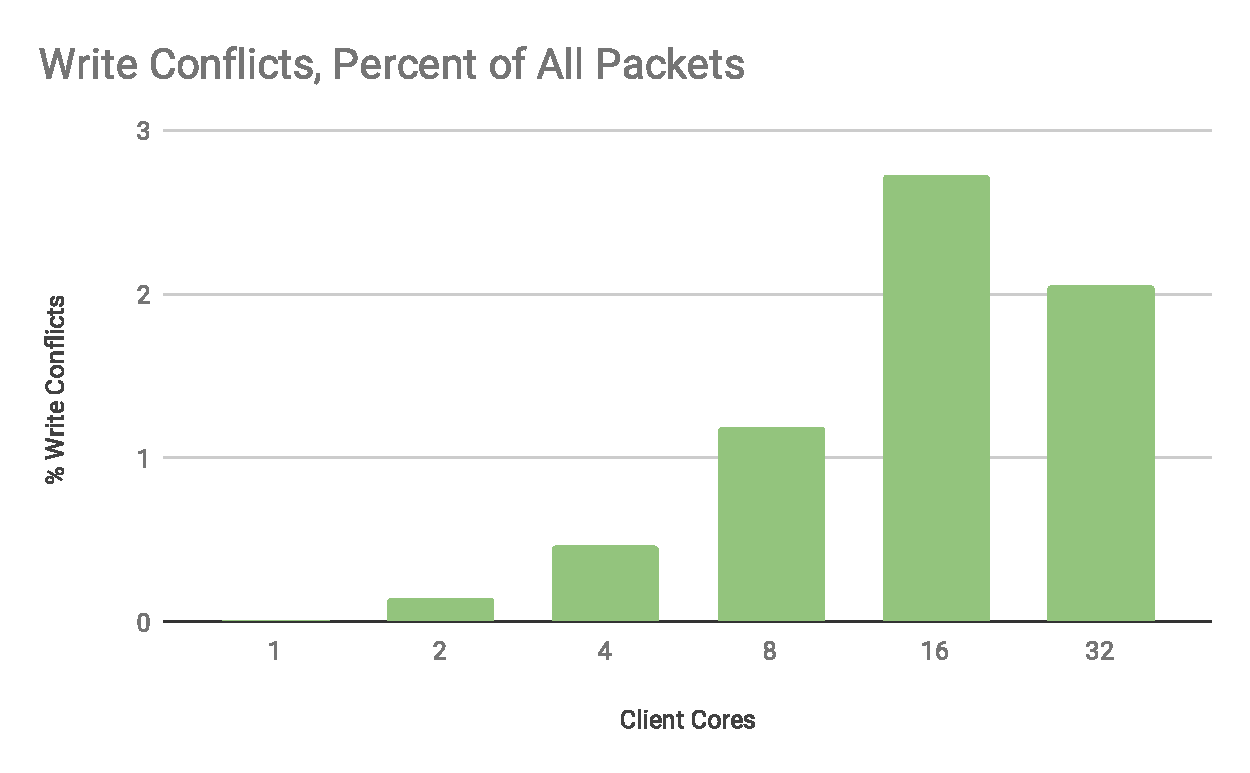
\includegraphics[width=0.45\textwidth]{fig/write_conflicts.pdf}
    \caption{Clover write conflicts grow with the number of clients
    (50\% write zipf 0.99 distribution)\todo{redo with 64 cores and
    writes only}}
    \label{fig:conflicts}
\end{figure}


In clovers specific case its throughput is severely degraded under
write heavy workloads. Figure~\ref{fig:clover_tput} shows clovers
reported throughput drop when subjected to a 50\% write workload.

\begin{figure}
    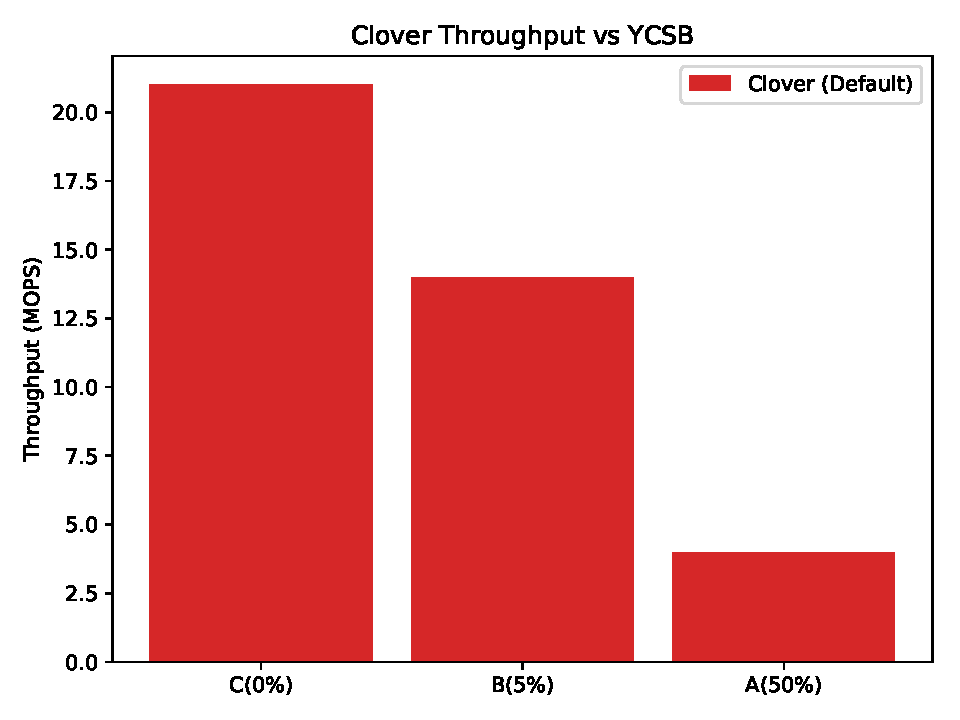
\includegraphics[width=0.45\textwidth]{fig/clover_tput.pdf}
    \caption{Clover throughput degradation as a function of write
    workload\todo{redo on my setup for consistent ops/s}}
    \label{fig:clover_tput}
\end{figure}

This work makes the contention that a programmable TOR is an ideal
centralized point at which to resolve remote memory conflicts. Prior
work has suggested the need for a distributed memory
controller~\cite{disandapp}, but none have been built or proposed with
existing hardware. We observe that in a disaggregated setting if all
remote reads and writes are performed within a rack using RDMA a TOR
in a unique position to observe every memory operation.  This fact
allows it to act as a centralized serialization point, where the last
instance of read/write concurrency are the memory attached egress
ports of the switch.  Figure~\ref{fig:overview} illustrates the
organization of a disaggregated rack, and highlights different
proposed points of coordination for reads and writes.

As a proof of concept we interpose on the Clover protocol and resolve
write conflicts in its datapath. Our conflict detection algorithm uses
knowledge of Clovers remote data structures to detect write conflicts
using a small amount of cached state (only a few bytes per key value
pair). Conflict resolution is performed directly on the in flight RDMA
packets by steering their destination virtual addresses to the most up
to date read and write locations in Clovers key value store. This
technique is complete, in that it resolves all read and write
conflicts given that it caches all keys. As in network SRAM is expense
we show that our technique can trade completeness for memory savings
while still achieving performance gains. Our preliminary evaluation
shows maximal throughput gains of 1.42x (tracking all reads and
writes), and gains of 1.34x when correcting conflicts on the top 8
keys of a zipf request distribution using only 128 bytes of in network
memory.
